\documentclass[tikz,border=10pt]{standalone}
% No extra TikZ libraries needed.
\begin{document}
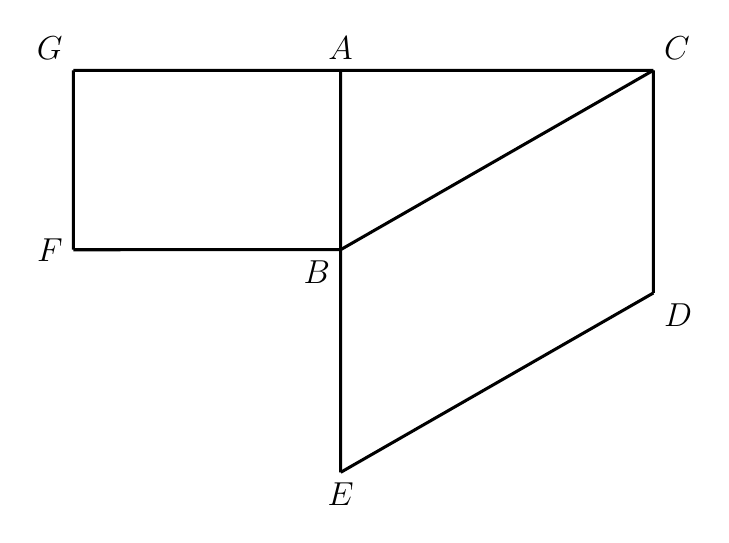
\begin{tikzpicture}[line width=1.1pt, line join=round, font=\fontsize{12}{14.4}\selectfont]
  % Scale s = 0.014388 cm/px, centre (338,256.5) px, y flipped
  \coordinate (G) at (-3.683546503420093,2.554720004638108);
  \coordinate (A) at (-0.2883091261807813,2.555438813042002);
  \coordinate (C) at (3.682988533474461,2.5562795796261764);
  \coordinate (F) at (-3.683064475793976,0.2778988041789907);
  \coordinate (B) at (-0.2878270985546646,0.2786176125828843);
  \coordinate (D) at (3.6835871512520897,-0.2712464235124348);
  \coordinate (E) at (-0.2872284807770362,-2.5489083905557264);

  % Segments
  \draw (G) -- (A) -- (C);   % top edge G-A-C
  \draw (G) -- (F);          % left edge
  \draw (F) -- (B);          % horizontal at y=237
  \draw (A) -- (E);          % vertical x=318, passes through B
  \draw (C) -- (B);          % diagonal C-B
  \draw (C) -- (D);          % right vertical
  \draw (D) -- (E);          % diagonal D-E

  % Labels outside each vertex
  \node[above left]  at (G) {$G$};
  \node[above]       at (A) {$A$};
  \node[above right] at (C) {$C$};
  \node[left]        at (F) {$F$};
  \node[below left]  at (B) {$B$};
  \node[below right] at (D) {$D$};
  \node[below]       at (E) {$E$};
\end{tikzpicture}
\end{document}
% GEOAGENT_REPAIR_V1 c18a466396f54661 99b0e4ba6736d63b8f2b83a4ebbe3a90af4dfb194574efeb9b985010317be364
